\documentclass{standalone}
\usepackage{tikz}
\usetikzlibrary{shapes,arrows,positioning,calc,automata,backgrounds}

\begin{document}
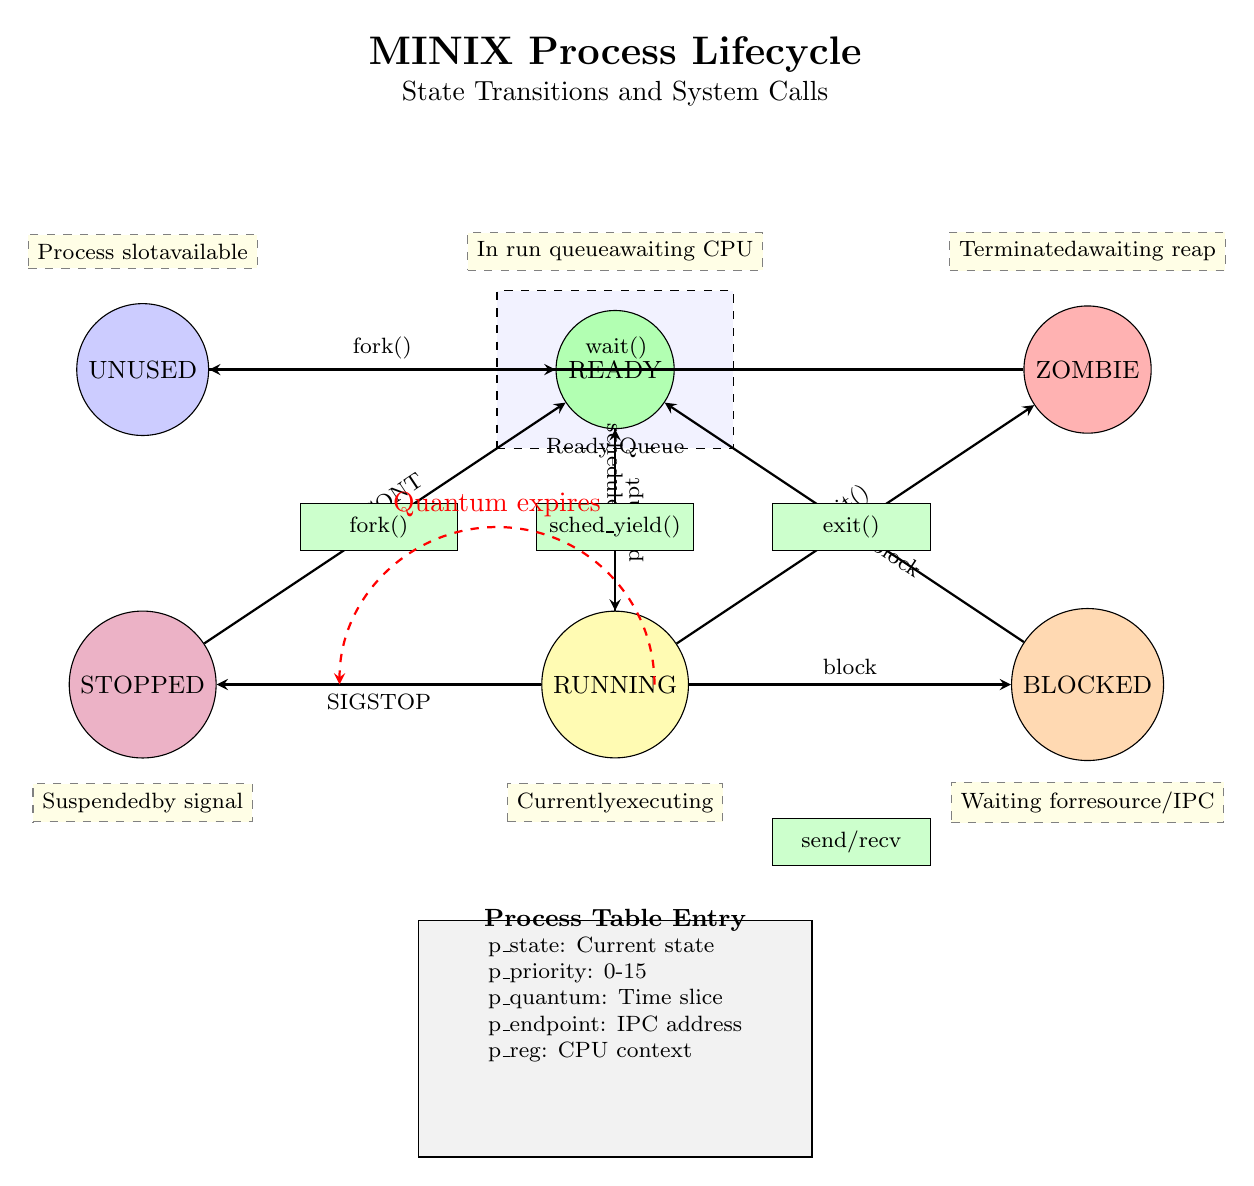
\begin{tikzpicture}[
    state/.style={circle, draw=black, fill=blue!20, minimum size=1.5cm, font=\small},
    trans/.style={rectangle, draw=black, fill=green!20, minimum width=2cm, minimum height=0.6cm, font=\footnotesize},
    arrow/.style={->, >=stealth, thick},
    label/.style={font=\footnotesize, sloped},
    note/.style={rectangle, draw=gray, dashed, fill=yellow!10, font=\footnotesize}
]

% Title
\node[font=\Large\bfseries] at (0, 8) {MINIX Process Lifecycle};
\node[font=\normalsize] at (0, 7.5) {State Transitions and System Calls};

% States
\node[state] (unused) at (-6, 4) {UNUSED};
\node[state, fill=green!30] (ready) at (0, 4) {READY};
\node[state, fill=yellow!30] (running) at (0, 0) {RUNNING};
\node[state, fill=orange!30] (blocked) at (6, 0) {BLOCKED};
\node[state, fill=red!30] (zombie) at (6, 4) {ZOMBIE};
\node[state, fill=purple!30] (stopped) at (-6, 0) {STOPPED};

% Transitions with labels
\draw[arrow] (unused) -- node[above, label] {fork()} (ready);
\draw[arrow] (ready) -- node[left, label] {schedule} (running);
\draw[arrow, bend right=30] (running) -- node[below, label] {preempt} (ready);
\draw[arrow] (running) -- node[above, label] {block} (blocked);
\draw[arrow] (blocked) -- node[right, label] {unblock} (ready);
\draw[arrow] (running) -- node[above, label] {exit()} (zombie);
\draw[arrow] (zombie) -- node[above, label] {wait()} (unused);
\draw[arrow] (running) -- node[below, label] {SIGSTOP} (stopped);
\draw[arrow] (stopped) -- node[above, label] {SIGCONT} (ready);

% Annotations
\node[note] at (-6, 5.5) {Process slot\\available};
\node[note] at (0, 5.5) {In run queue\\awaiting CPU};
\node[note] at (0, -1.5) {Currently\\executing};
\node[note] at (6, -1.5) {Waiting for\\resource/IPC};
\node[note] at (6, 5.5) {Terminated\\awaiting reap};
\node[note] at (-6, -1.5) {Suspended\\by signal};

% Process Table Entry box
\node[rectangle, draw=black, fill=gray!10, minimum width=5cm, minimum height=3cm] (ptable) at (0, -4.5) {};
\node[font=\small\bfseries] at (0, -3) {Process Table Entry};
\node[font=\footnotesize, align=left] at (0, -4) {
    p\_state: Current state\\
    p\_priority: 0-15\\
    p\_quantum: Time slice\\
    p\_endpoint: IPC address\\
    p\_reg: CPU context
};

% System calls that trigger transitions
\node[trans] at (-3, 2) {fork()};
\node[trans] at (3, 2) {exit()};
\node[trans] at (0, 2) {sched\_yield()};
\node[trans] at (3, -2) {send/recv};

% Scheduling queues visualization
\begin{scope}[on background layer]
    \node[rectangle, draw=black, dashed, fill=blue!5, minimum width=3cm, minimum height=2cm] at (0, 4) {};
\end{scope}
\node[font=\footnotesize] at (0, 3) {Ready Queue};

% Time quantum annotation
\draw[arrow, red, dashed] (0.5, 0) arc (0:180:2cm) node[midway, above] {Quantum expires};

\end{tikzpicture}
\end{document}